\begin{figure}[ht]
\centering
%%%%%%%%%%%%%%%% left: the strictly-signed nodes
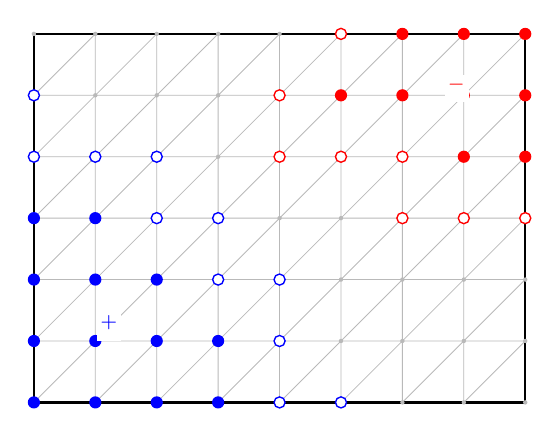
\begin{tikzpicture}[x=0.78cm,y=0.78cm]
  \draw[gray!55,line width=0.3pt]
    \foreach \i in {0,...,8} {(\i,0) -- (\i,6)}
    \foreach \j in {0,...,6} {(0,\j) -- (8,\j)}
    \foreach \i in {0,...,7} {\foreach \j in {0,...,5} {(\i,\j) -- ({\i+1},{\j+1})}};
  \draw[thick] (0,0) rectangle (8,6);
  \foreach \i/\j in {0/6, 1/5, 1/6, 2/5, 2/6, 3/4, 3/5, 3/6, 4/3, 4/6, 5/1, 5/2, 5/3, 6/0, 6/1, 6/2, 7/0, 7/1, 7/2, 8/0, 8/1, 8/2}
    \fill[gray!55] (\i,\j) circle (0.8pt);
  \foreach \i/\j in {0/4, 0/5, 1/4, 2/3, 2/4, 3/2, 3/3, 4/0, 4/1, 4/2, 5/0}
    \draw[Blue,line width=0.5pt,fill=white] (\i,\j) circle (2.0pt);
  \foreach \i/\j in {4/4, 4/5, 5/4, 5/6, 6/3, 6/4, 7/3, 8/3}
    \draw[Red,line width=0.5pt,fill=white] (\i,\j) circle (2.0pt);
  \foreach \i/\j in {0/0, 0/1, 0/2, 0/3, 1/0, 1/1, 1/2, 1/3, 2/0, 2/1, 2/2, 3/0, 3/1}
    \fill[Blue] (\i,\j) circle (2.2pt);
  \foreach \i/\j in {5/5, 6/5, 6/6, 7/4, 7/5, 7/6, 8/4, 8/5, 8/6}
    \fill[Red] (\i,\j) circle (2.2pt);
  \node[Blue,fill=white,inner sep=1pt] at (1.23,1.23) {$\Nh^+$};
  \node[Red,fill=white,inner sep=1pt] at (6.89,5.11) {$\Nh^-$};
\end{tikzpicture}
\hfill
%%%%%%%%%%%%%%%% right: their star dilations
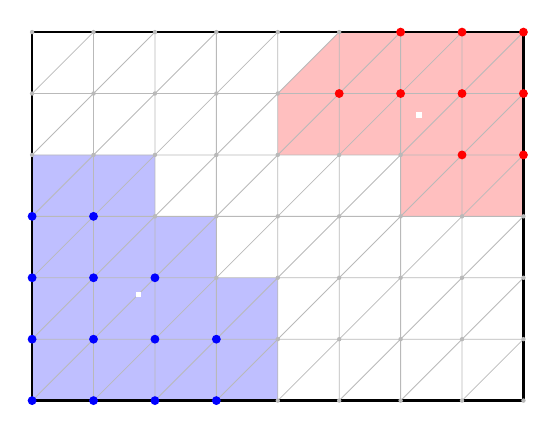
\begin{tikzpicture}[x=0.78cm,y=0.78cm]
  \foreach \i/\j in {0/0, 0/1, 0/2, 0/3, 1/0, 1/1, 1/2, 1/3, 2/0, 2/1, 2/2, 3/0, 3/1}
    \fill[Blue!25] (\i,\j) -- ({\i+1},\j) -- ({\i+1},{\j+1}) -- cycle;
  \foreach \i/\j in {0/0, 0/1, 0/2, 0/3, 1/0, 1/1, 1/2, 1/3, 2/0, 2/1, 2/2, 3/0, 3/1}
    \fill[Blue!25] (\i,\j) -- ({\i+1},{\j+1}) -- (\i,{\j+1}) -- cycle;
  \foreach \i/\j in {4/4, 4/5, 5/4, 5/5, 6/3, 6/4, 6/5, 7/3, 7/4, 7/5}
    \fill[Red!25] (\i,\j) -- ({\i+1},\j) -- ({\i+1},{\j+1}) -- cycle;
  \foreach \i/\j in {4/4, 5/4, 5/5, 6/3, 6/4, 6/5, 7/3, 7/4, 7/5}
    \fill[Red!25] (\i,\j) -- ({\i+1},{\j+1}) -- (\i,{\j+1}) -- cycle;
  \draw[gray!55,line width=0.3pt]
    \foreach \i in {0,...,8} {(\i,0) -- (\i,6)}
    \foreach \j in {0,...,6} {(0,\j) -- (8,\j)}
    \foreach \i in {0,...,7} {\foreach \j in {0,...,5} {(\i,\j) -- ({\i+1},{\j+1})}};
  \draw[thick] (0,0) rectangle (8,6);
  \foreach \i/\j in {0/4, 0/5, 0/6, 1/4, 1/5, 1/6, 2/3, 2/4, 2/5, 2/6, 3/2, 3/3, 3/4, 3/5, 3/6, 4/0, 4/1, 4/2, 4/3, 4/4, 4/5, 4/6, 5/0, 5/1, 5/2, 5/3, 5/4, 5/6, 6/0, 6/1, 6/2, 6/3, 6/4, 7/0, 7/1, 7/2, 7/3, 8/0, 8/1, 8/2, 8/3}
    \fill[gray!55] (\i,\j) circle (0.8pt);
  \foreach \i/\j in {0/0, 0/1, 0/2, 0/3, 1/0, 1/1, 1/2, 1/3, 2/0, 2/1, 2/2, 3/0, 3/1}
    \fill[Blue] (\i,\j) circle (1.6pt);
  \foreach \i/\j in {5/5, 6/5, 6/6, 7/4, 7/5, 7/6, 8/4, 8/5, 8/6}
    \fill[Red] (\i,\j) circle (1.6pt);
  \node[Blue,fill=white,inner sep=1pt] at (1.73,1.73) {$\ombot$};
  \node[Red,fill=white,inner sep=1pt] at (6.30,4.65) {$\omtop$};
\end{tikzpicture}
\caption{The strictly-signed nodal sets and their star dilations, on the mesh of Figure~\ref{fig:nodalelem}.  Left: $\Nh^+$ and $\Nh^-$ from \eqref{eq:Nhpm} as filled dots, with the remaining nodes of $\Nhbot$ and $\Nhtop$, where $\sigma_h$ vanishes, as open circles.  Right: the star dilations $\ombot = \Uh(\Nh^+)$ and $\omtop = \Uh(\Nh^-)$ from \eqref{eq:omegas}, each one ring of elements larger than the node set generating it.  Which active nodes carry a strict sign is notional here.}
\label{fig:stardilate}
\end{figure}
